\chapter{Funkcja celu -- porównanie barwy dźwięku}~\label{target_function_chapter}

Aby stopniowo dostosować graf przetwarzania sygnałów zaimplementowany 
w rozdziale~\ref{dsp_graph_chapter} do imitowania zadanej próbki dźwięku,
należy wykorzystać funkcję celu, która maleje wraz ze wzrostem podobieństwa
barwy dźwięku między próbki zadaną i sygnałem generowanym przez graf. 

\begin{figure}[H]\label{fig:waveform_not_equal_to_perception}
    \centering
    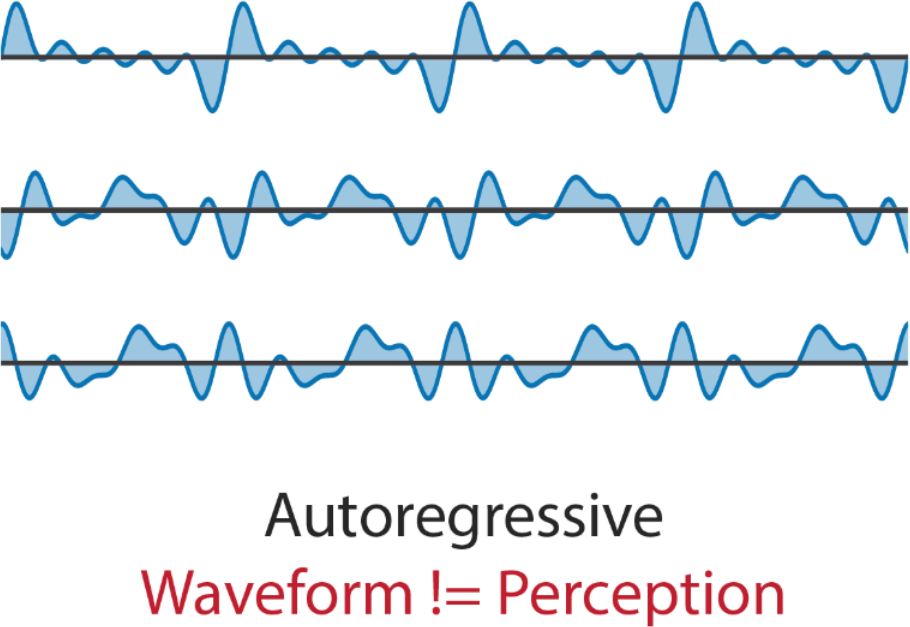
\includegraphics[width=0.45\linewidth]{rys03/d_dsp_example_graph.png}
    \caption{
      Przykład trzech próbek dźwięku, które dla słuchacza brzmią identycznie, mimo
      znacznych różnic w kształcie fali. Źródło obrazka:~\cite{engel2020ddsp}.
    }
\end{figure}

\section{Porównanie barwy dźwięku w literaturze}\label{sec:timbre_comparison_literature_overview}

Żadna z prac przeanalizowanych podczas przeglądu literatury
(\cite{engel2020ddsp},~\cite{ieee_synth_programming},~\cite{ddx7},~\cite{riffusion},~\cite{evolutionary_puredata},~\cite{parallel_evolutionary_optimization_synth_parameters},~\cite{mfcc_dtw})
nie wykorzystuje metod porównywania sygnału osadzonych jedynie w dziedzinie czasu, ponieważ
nie są one skuteczne do porównywania dźwięków pod względem odczuć psychoakustycznych.
Przykład różnych kształtów fali, które z perspektywy słuchacza brzmią jak
taki sam dźwięk zademonstrowano na rysunku~\ref{fig:waveform_not_equal_to_perception}.

Ponieważ porównywanie barwy dźwięku instrumentów muzycznych nie należy do popularnych
tematów badań, podczas przeglądu literatury wykorzystano również badania dotyczące
rozpoznawania głosu, wykorzystujące współczynniki MFCC oraz
\textit{dynamic time warping}~(DTW)~\cite{mfcc_dtw}.

\subsection{Systematyzacja metod z literatury}~\label{sec:timbre_comparison_systematisation}

Metody zaczerpięte z literatury wykorzystują różne podejścia do porównywania barwy dźwięku
pomiędzy sygnałami. Podejścia te można usystematyzować za pomocą dwóch cech:

\begin{enumerate}
  \item Rodzaj wykonanej transformacji z dziedziny czasu do dziedziny częstotliwości:
  \begin{itemize}
    \item transformata Fouriera (w różnych konfiguracjach)~\cite{riffusion}~\cite{ddx7},
    \item MFCC~\cite{ieee_synth_programming}~\cite{evolutionary_puredata}~\cite{mfcc_dtw}.
  \end{itemize}
  \item Dalsze przetwarzanie reprezentacji sygnału w domenie częstotliwości, w celu ułatwienia optymalizacji:
    \begin{itemize}
      \item dostosowywanie wagi konkretnych próbek na podstawie metryki określającej siłę sygnału
        (na przykład \textit{root-mean-square}, RMS)~\cite{parallel_evolutionary_optimization_synth_parameters},
        aby wzmocnić istotność głośniejszych fragmentów dźwięku,
      \item wykorzystanie \textit{dynamic time warping}, aby funkcja celu przyzwalała na
        niedokładności w odwzorowaniu dokładnej dynamiki zmian w charakterystyce spektralnej~\cite{mfcc_dtw}.
    \end{itemize}
\end{enumerate}

\subsection{Wybór funkcji celu do przetestowania}~\label{sec:considered_target_functions}

Na podstawie analizy metod z literatury opisanej w rozdziale~\ref{sec:timbre_comparison_systematisation} zostały wybrane wszystkie warianty
funkcji celu wykorzystywane w przeanalizowanej literaturze:

\begin{enumerate}
  \item Różnica w spektrum Fouriera,
  \item Różnica w spektrum Fouriera liczona za pomocą DTW,
  \item Różnica w MFCC,
  \item Różnica w MFCC liczona za pomocą DTW\@,
  \item Różnica w MFCC ważonym za pomocą RMS\@.
\end{enumerate}

\section{Proces testowania funkcji celu}

\begin{figure}[H]\label{fig:fm_graph_for_benchmarks}
    \centering
    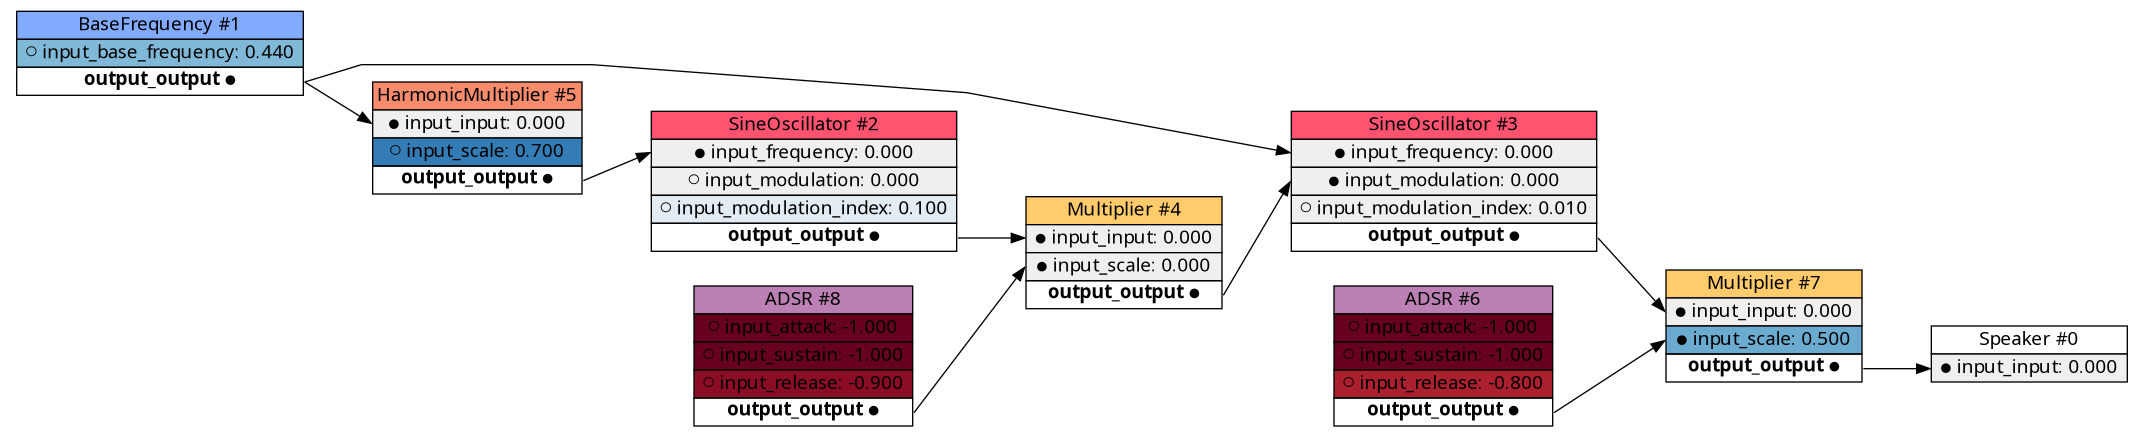
\includegraphics[width=1.0\linewidth]{rys03/fm_graph_for_benchmarks.png}
    \caption{
      Prosty graf syntezy FM, zawierający jeden oscylator służący za sygnał nośny
      i jeden oscylator służący za sygnał modulujący.
    }
\end{figure}

Metoda testowania została zaczerpnięta z~\cite{evolutionary_puredata}.
Funkcje celu zostały wpierw przetestowane poprzez wykonanie
zbioru przekrojów przez uproszczony problem syntezy typu FM\@.
Następnie przeprowadzono próby automatycznego dostosowania parametrów dwóch grafów
o predefiniowanej strukturze, dla syntezy FM oraz \textit{analog modeling}.

\section{Przekrój wartości funkcji celu dla prostego problemu syntezy typu FM}\label{sec:fm_synth_params_cross_section}

Testy obejmowały wygenerowanie wartości funkcji celu podczas
modyfikowania pojedynczego parametru w grafie przetwarzania sygnałów
przedstawionym na rysunku~\ref{fig:fm_graph_for_benchmarks}.
Modyfikowane parametry odpowiadają za różne cechy barwy uzyskanego dźwięku:

\begin{itemize}
  \item \texttt{HarmonicMultiplier/input\_scale}: częstotliwość modulacji FM,
  \item \texttt{SineOscillator/input\_modulation\_index}: siła składowych harmonicznych,
  \item \texttt{ADSR/input\_attack}: dynamika dźwięku.
\end{itemize}


\begin{figure}[H]\label{fig:target_function_testing}
    \centering
    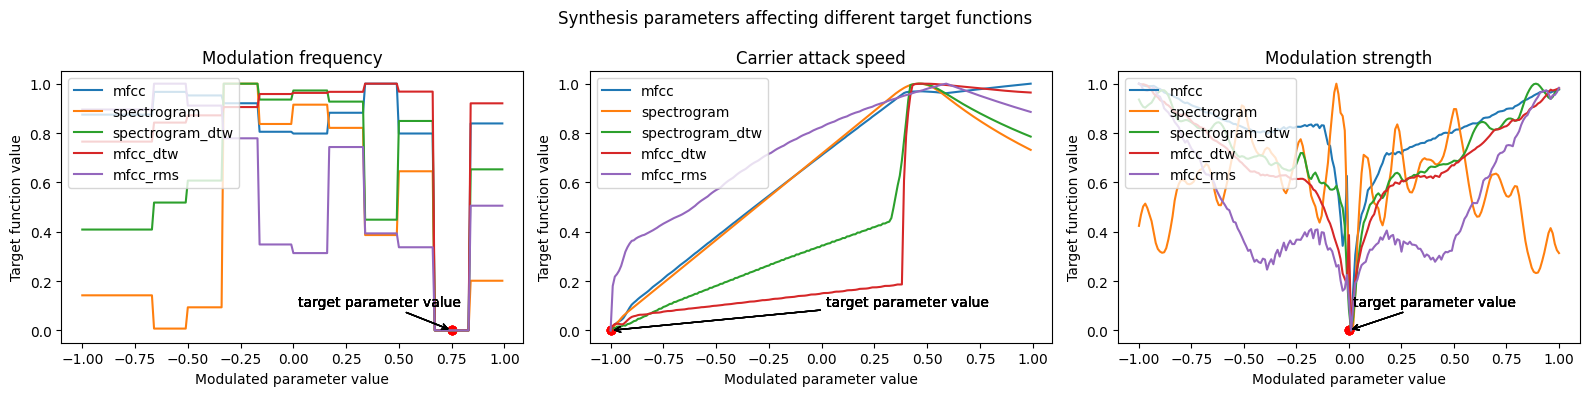
\includegraphics[width=1.0\linewidth]{rys03/target_function_testing.png}
    \caption{
      Zmiany w wartościach testowanych funkcji celu podczas przesuwania różnych parametrów syntezy dźwięku. 
      Kształt pierwszego wykresu wynika z zastosowania kwantyzacji dostępnych częstotliwości modulacji,
      aby wykluczyć nieharmoniczne stosunki częstotliwości modulacji i nośnej. Tego rodzaju praktyka
      jest wykorzystywana w syntezatorach FM~\cite{digitone_manual}, ponieważ ułatwia dostosowywanie parametrów syntezy.
    }
\end{figure}

\subsection{Analiza wyników}

Wyniki testów zaprezentowane na wykresach~\ref{fig:target_function_testing} pozwalają na
wyeliminowanie różnicy między spektrogramami jako funkcji celu,
ponieważ w przypadku zmian częstotliwości modulacji posiada ona minimum globalne w 
niewłaściwej pozycji parametru. Późniejsze testy wykorzystują tylko funkcje celu
wykorzystujące MFCC\@.

\subsubsection{Częstotliwość modulacji FM}

Wszystkie funkcje z wyjątkiem różnicy między spektrogramami pokazują poprawną, 
najniższą wartość dla właściwej wartości parametru.

\subsubsection{Dynamika dźwięku}

W przypadku wpływu zmian w dynamice dźwięku na wartości funkcji celu,
zastosowanie DTW znacząco zmienia kształt funkcji celu, zależnie od wybranego rozmiaru
okna DTW\@. Duży rozmiar okna powoduje zmniejszenie kary za niedokładne odwzorowanie
dynamiki dźwięku. 

\subsubsection{Siła modulacji}

Różnica między spektrogramami jest najbardziej chaotyczna, nie maleje wraz
ze zbliżaniem się do poprawnej wartości parametru. Pozostałe funkcje celu
wykorzystujące \textit{MFCC} mają lepszą charakterystykę -- maleją
wraz ze zbliżaniem się do poprawnej wartości parametru.

\section{Optymalizacja parametrów dla predefiniowanych
grafów syntezy FM oraz \textit{analog modeling}}

Drugą częścią procesu testowania funkcji celu z literatury było zweryfikowanie skuteczności
każdej z funkcji w uproszczonym problemie optymalizacyjnym, polegającym jedynie na odnalezieniu właściwych
parametrów dla predefiniowanej struktury grafu DSP\@. Wykorzystano dwa grafy
DSP~(\ref{fig:analog_graph_for_benchmarks},~\ref{fig:fm_graph_for_benchmarks}),
wykonujące różne rodzaje syntezy.


\subsection{Synteza FM}

Testowana struktura grafu wykonującego syntezę typu FM~\ref{fig:fm_graph_for_benchmarks}
wykorzystuje 2 operatory: jedną nośną
i jeden modulator. Parametry grafu zostały ręcznie dostrojone aby wygenerować krótki
dźwięk typu \textit{pluck}, w którym modulator przekształca nośną sinusoidę w sygnał zbliżony
do sygnału prostokątnego. Z perspektywy wynikowego spektrum sygnału, przedstawionego na
rysunku~\ref{fig:param_optimisation_results_spectrograms} sygnał składa się z częstotliwości
podstawowej i jednej składowej harmonicznej. Wizualizacja sygnału została przedstawiona
na wykresie~\ref{fig:fm_training_sample_overview}.

\begin{figure}[H]
    \centering
    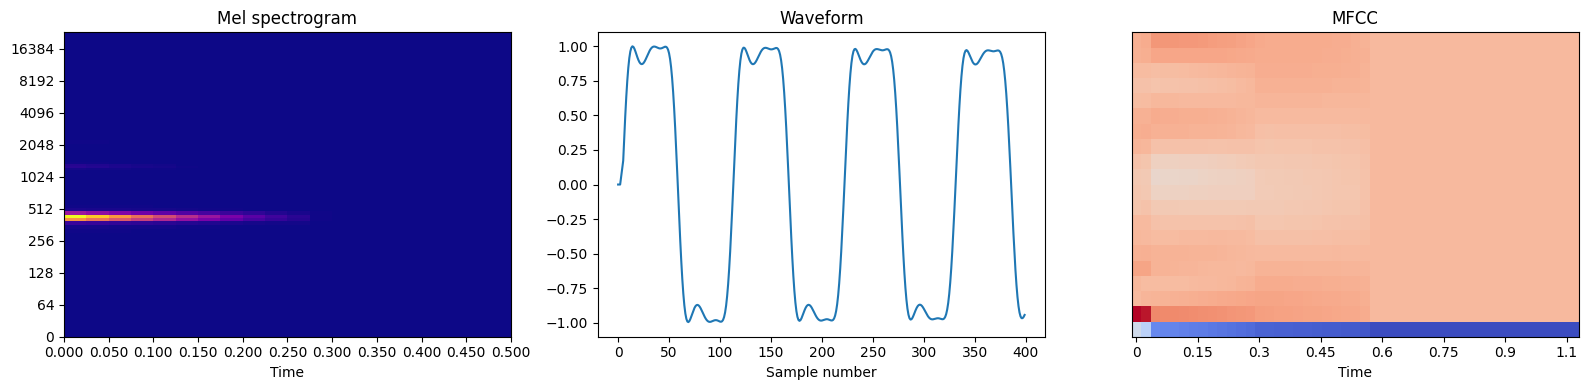
\includegraphics[width=1.0\linewidth]{rys03/fm_training_sample_overview.png}
    \caption{
      Spektrogram, kształt fali oraz wizualizacja MFCC dla próbki dźwięku, którą
      ma imitować graf syntezy FM podczas testów różnych funkcji celu.
    }\label{fig:fm_training_sample_overview}
\end{figure}


\subsection{Synteza \textit{analog modeling}}

\begin{figure}[H]
    \centering
    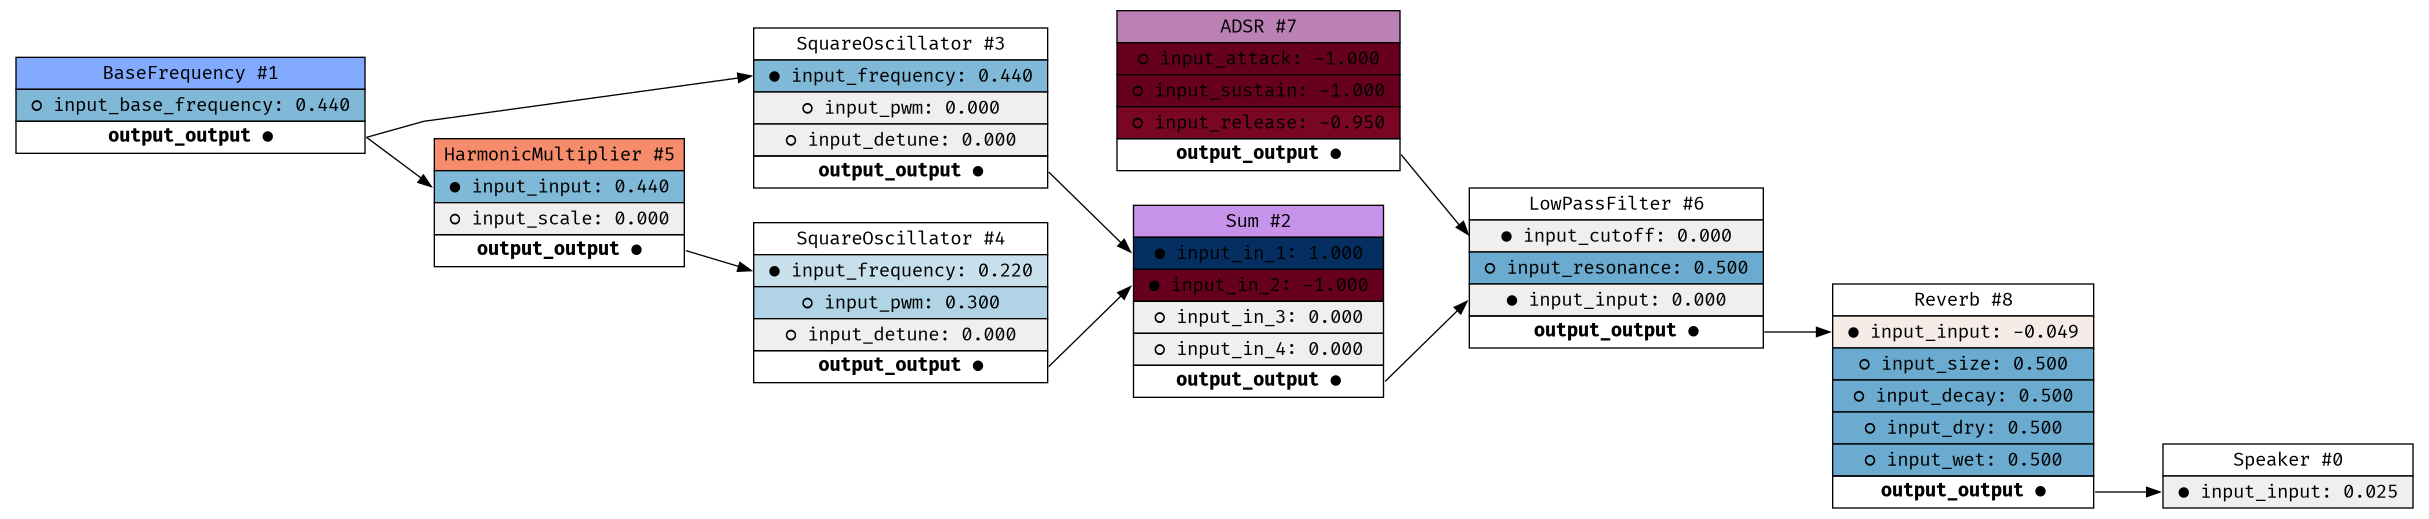
\includegraphics[width=1.0\linewidth]{rys03/analog_graph_for_benchmarks.png}
    \caption{
      Graf wykonujący syntezę typu \textit{analog modeling}, wykorzystany do testów funkcji celu.
    }\label{fig:analog_graph_for_benchmarks}
\end{figure}

Synteza \textit{analog modeling} zazwyczaj wykorzystuje więcej parametrów niż synteza
FM~(\ref{fig:fm_graph_for_benchmarks}), aby zwiększyć trudność problemu optymalizacyjnego
graf został roszszerzony o węzeł dodający efekt pogłosu~\cite{reverb}.
Struktura grafu (przedstawiona na rysunku~\ref{fig:analog_graph_for_benchmarks}) składa
się z dwóch oscylatorów generujących sygnał prostokątny. Oscylator \texttt{SquareOscillator \#4}
generuje sygnał przesunięty o oktawę w dół w stosunku do częstotliwości podstawowej, jednocześnie
jego parametr \texttt{input\_pwm} skraca szerokość generowanego impulsu, aby wzbogacić barwę dźwięku
o dodatkowe składowe harmoniczne. Barwa dźwięku zmienia się dynamicznie w czasie dzięki 
zastosowaniu filtra niskoprzepustowego (\texttt{LowPassFilter \#6}), którego
częstotliwość odcięcia jest modulowana przez sygnał sterujący \texttt{ADSR \#7}.
Długość dźwięku generowanego przez oscylatory jest podobna jak w przypadku
grafu FM~(\ref{fig:fm_graph_for_benchmarks}), zastosowanie węzła \texttt{Reverb \#8}
przedłuża czas trwania dźwięku i dodatkowo~,,rozmywa go'' w czasie, co pokazuje
spektrum sygnału na wykresie~\ref{fig:am_training_sample_overview}.

\begin{figure}[H]
  \centering
  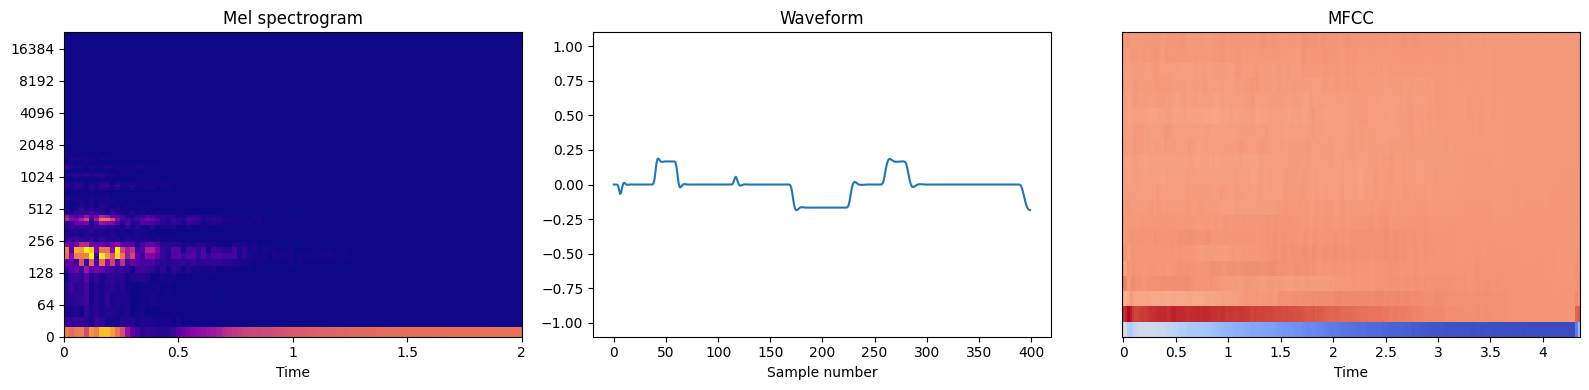
\includegraphics[width=1.0\linewidth]{rys03/am_training_sample_overview.png}
  \caption{
    Spektrogram, kształt fali oraz wizualizacja MFCC dla próbki dźwięku, którą
    ma imitować graf syntezy \textit{analog\_modeling} podczas testów różnych funkcji celu.
  }\label{fig:am_training_sample_overview}
\end{figure}



\subsection{Plan testów}

Dla obu grafów wykonano optymalizację parametrów wejściowych w celu imitacji danej
próbki dźwięku. Optymalizację wykonano 10 razy dla każdej rozważanej~(\ref{sec:considered_target_functions})
funkcji celu. Do optymalizacji parametrów wykorzystano algorytm evolucyjny
\textit{differential evolution}~\cite{2020SciPy-NMeth}.

\subsection{Wyniki testów}

\begin{figure}[H]
    \centering
    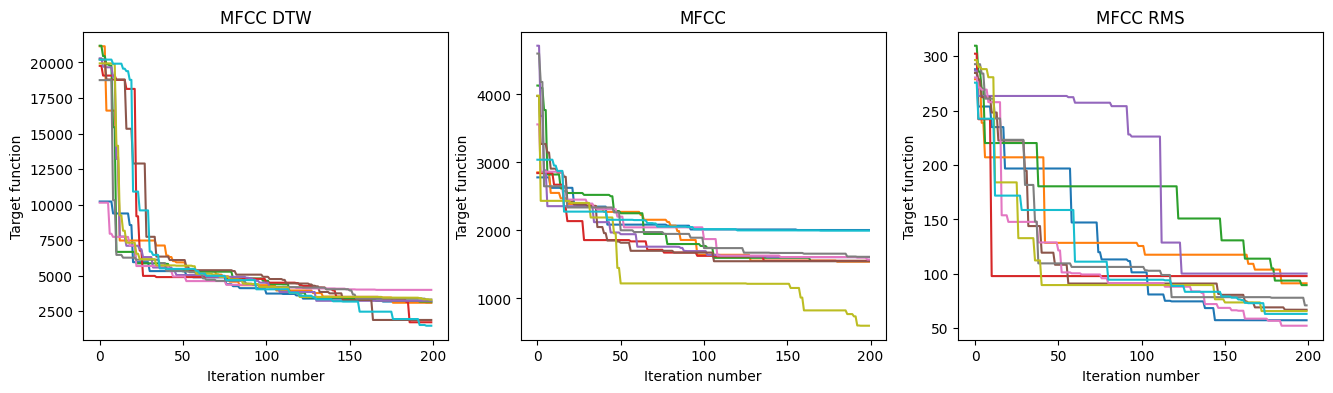
\includegraphics[width=1.0\linewidth]{rys03/target_functions_progress.png}
    \caption{
      Wykresy zmian funkcji celu podczas optymalizacji dla grafu syntezy FM\@.
    }\label{fig:param_optimisation_results_target_fun_plots}
\end{figure}

\begin{figure}[H]
    \centering
    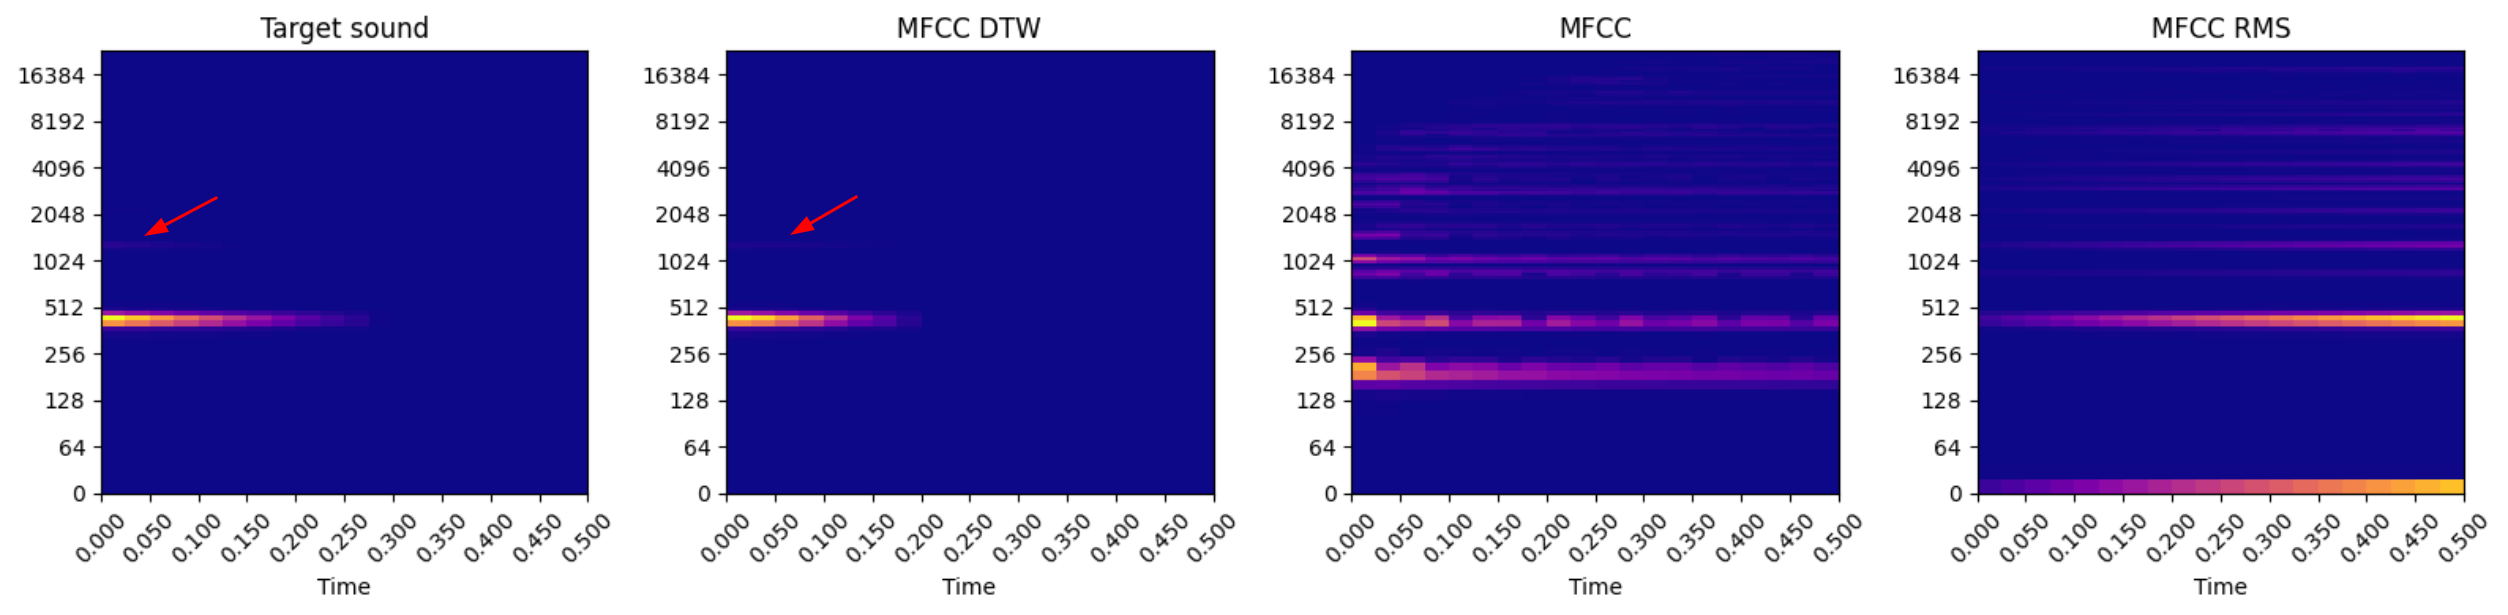
\includegraphics[width=1.0\linewidth]{rys03/spectro_results_fm.png}
    \caption{
      Spektrogram dźwięku docelowego oraz dźwięków uzyskanych w procesie optymalizacji parametrów grafu FM\@.
      Czerwoną strzałką oznaczono składową harmoniczną (słabo widoczną na spektrogramie),
      która została poprawnie odtworzona przez algorytm optymalizacji.
    }\label{fig:param_optimisation_results_spectrograms}
\end{figure}

\subsubsection{Synteza FM}

Algorytm optymalizacji jest w stanie poprawnie dostosować wartości parametrów grafu w przypadku
zastosowania MFCC+DTW jako funkcji celu. Jak pokazuje spektrogram~(\ref{fig:param_optimisation_results_spectrograms}),
poprawnie odtworzona jest zarówno dynamika dźwięku i składowa harmoniczna. Pozostałe funkcje celu nie pozwalają
na odtworzenie sygnału, który w bliski sposób przypomina dźwięk docelowy, pomimo uzyskiwania wyników zbliżonych
do MFCC+DTW we wcześniejszych testach~(\ref{sec:fm_synth_params_cross_section}).

\subsubsection{Synteza \textit{analog modeling}}

\begin{figure}[H]
    \centering
    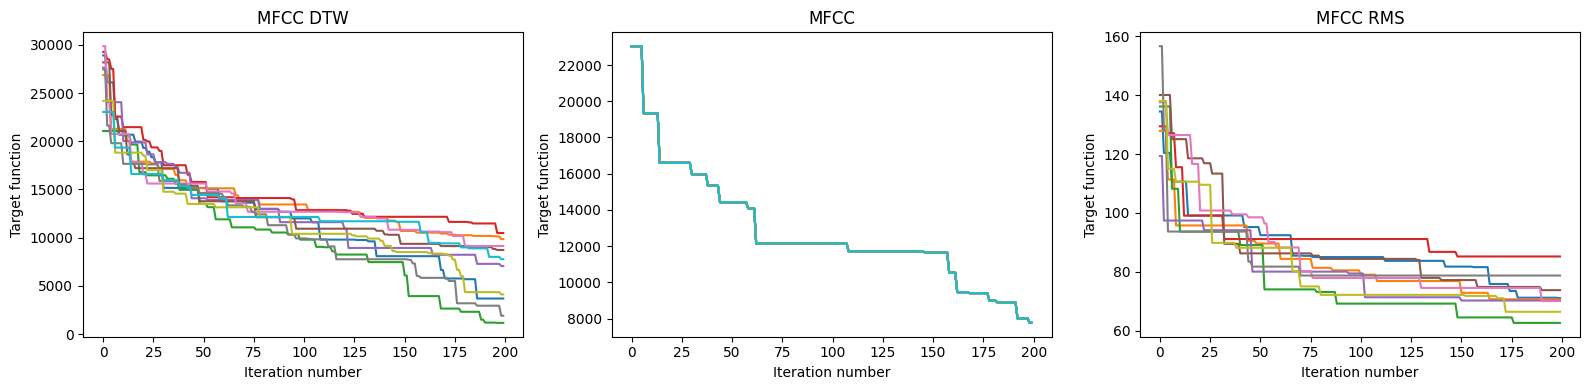
\includegraphics[width=1.0\linewidth]{rys03/am_training_results.png}
    \caption{
      Wykresy zmian funkcji celu podczas optymalizacji dla grafu syntezy \textit{analog modeling}.
      \textbf{TODO\@: pełny wykres}.
    }\label{fig:am_target_fun_plots}
\end{figure}

\begin{figure}[H]
    \centering
    % 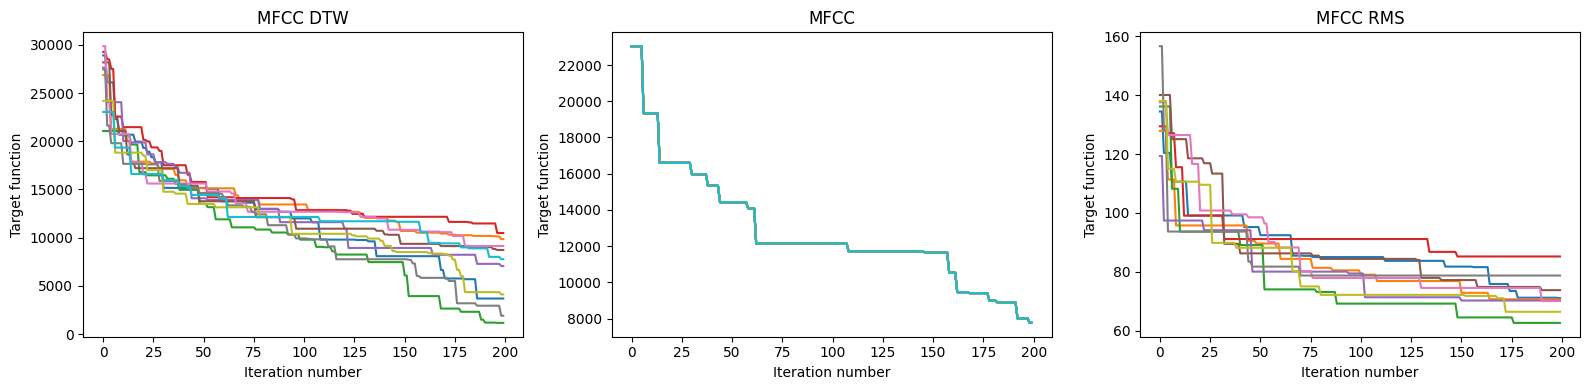
\includegraphics[width=1.0\linewidth]{rys03/am_spectro_results.png}
    \caption{
      Spektrogram dźwięku docelowego oraz dźwięków uzyskanych w procesie
      optymalizacji parametrów grafu \textit{analog modeling}.
      \textbf{TODO\@: obrazek}.
    }\label{fig:am_param_optimisation_results_spectrograms}
\end{figure}

Podobnie jak podczas testów syntezy FM, funkcja celu MFCC+DTW pozwala na dokładne odwzorowanie barwy dźwięku.
Na spektrogramie~(\ref{fig:am_param_optimisation_results_spectrograms}) widoczne są poprawnie odtworzone
składowe harmoniczne, przebieg dynamiczny dźwięku oraz parametry efektu pogłosu.
\textbf{Tutaj trzeba dodać więcej tekstu i spektrogramy jak się już przekręci cała optymalizacja.}

\subsection{Wybór funkcji celu na podstawie wyników}

Wyniki testów pozwalają jednoznacznie wybrać funkcję celu, która porównuje wartości MFCC
sygnałów za pomocą algorytmu \textit{dynamic time warping}. W zakresie pracy nie leży szczegółowe
wytłumaczenie, czemu zastosowanie DFT usprawnia proces optymalizacji. Możliwym intuicyjnym
wytłumaczeniem tego fenomenu jest fakt, że DFT pozwala na rozpoznanie poszczególnych
fonemów w nagraniach mowy~\cite{mfcc_dtw}, niezależnie od prędkości wypowiadania słów. 
Analogicznie, w przypadku porównywania sygnałów dźwiękowych generowanych przez grafy
przetwarzania sygnałów, wykorzystanie DFT może powodować~,,wygładzenie'' niedokładności
w zmianach tembru (transjentach~\cite{transient_music_theory}) i dynamiki dźwięku,
które występują pomiędzy sygnałem docelowym i wygenerowanym.
